% /* cSpell:enable */
% /* cSpell:locale de,en */
\chapter{Maßnahmen und Strategieen}
\label{cha:daten}

\section{Methodik}
\label{sec:datasets}

Als priorisierter Datensatz wurde das Angebot "Our World in Data" des Global Change Data Labs aus Großbritannien herangezogen. Die Organisation sammelt seit Pandemiebeginn Daten aus über 200 Ländern und bietet diese täglich aktualisiert zur freien Verwendung an. Pandemiedaten wie Fallzahlen, Todesfälle, Spitalsbelegungen und Testzahlen werden aus verschiedenen Quellen, unter anderem der nationalen Regierungen, dem European Centre for Disease Prevention and Control (ECDC), der Johns Hopkins University, gesammelt. Ergänzt werden diese unter anderem durch Daten wie Bruttoinlandsprodukt, durchschnittliche Lebenserwartung und Gesundheitsdaten von der Organisation for Economic Cooperation and Development (OECD) und der Weltbank, um eine demographische Beschreibung der Bevölkerung zur Verfügung zu stellen. \cite{owidcoronavirus}

Aus diesem Datensatz ist der "Stringency Index", ein errechneter Wert zwischen Null und 100, der Maßnahmen wie Schulschließungen, Versammlungsbeschränkungen, Reisebeschränkungen, Ausgangsbeschränkungen und Verordnungen an Arbeitsplätzen vergleicht und bewertet. Dabei sei betont, dass es sich bei diesem Wert um keine Beschreibung der Wirksamkeit der Maßnahmen handelt, sondern dieser nur zum Vergleich verschiedener Regionen und Staaten dient. \cite{oxcgrt}

Für Deutschland wurden zudem Daten des Projektes "Die Corona-Datenplattform" -- ein vom deutschem Bundesministerium für Wirtschaft und Klimaschutz in Auftrag gegebenes Projekt -- genutzt. Dieser Datensatz bietet im Vergleich zu "Our World in Data" eine genauere Auflösung, welche Maßnahmen genau gegolten haben und ist auch feingranularer bezüglich der exakt verimpften Impfstoffe. \cite{coronadatenplattform_de}

Für Österreich wurden die Daten aus dem COVID-19 Open Data Informationsportal genutzt. \cite{opendata_at}

Im Rahmen dieser Arbeit wurde die Datensatz-Beschreibung für den Datensatz von "Our World in Data" neu aufbereitet und für die verschiedenen Quellen ein Python-Skript mit Jupyter Code Cells als Schnittstelle zur Datenabfrage und Ausgabe erstellt. Dieses ist frei auf GitHub verfügbar.

\section{Ergebnisse}

Im folgenden wurde versucht, eine Korrelation zwischen Fallzahlen, Todesfällen, Maßnahmen (Stringency Index) und Impfzahlen zu finden. Verwendet wurden dazu die Korrelationskoeffizienten von Bravais-Pearson.

\subsection{Korrelation zwischen Fallzahlen und Todesfällen}

Betrachtet man die Todesfälle und die Fallzahlen, so fällt auf, dass diese Daten in Österreich und Deutschland miteinander korrelieren, in Großbritannien und Schweden ist dieser Effekt auch zu beobachten, jedoch schwächer ausgeprägt. Generell nahm diese Korrelation zwischen Fallzahlen und Todesfällen im Verlauf der Pandemie in Europa deutlich ab (siehe Tabellen in Anhang \ref{app:tabellen}). Im folgenden wurden speziell die Länder Österreich, Deutschland, Großbritannien und Schweden genauer untersucht.

\subsection{Maßnahmen zur Eindämmung der Pandemie}
\label{sec:massnahmen}

Der Stringency Index (s. Abbildung \ref{fig:stringency_index_comparison}) zeigt die in Kapitel \ref{sec:pandemieverlauf} erwähnten erlassenen und ausgesetzten Maßnahmen. Hier ist deutlich zu sehen, dass den Ruf, den Schweden hatte -- auf recht lockere Maßnahmen zu setzen -- nur bedingt wahr ist. Es wurden zwar lockerere Maßnahmen erlassen, diese dafür länger beibehalten. 
In Österreich und Deutschland wurden strengere Maßnahmen erlassen, welche aber schneller aufgehoben wurden.

\begin{figure}[ht]
    \caption{Stringency Index}
    \label{fig:stringency_index_comparison}
    \centering
    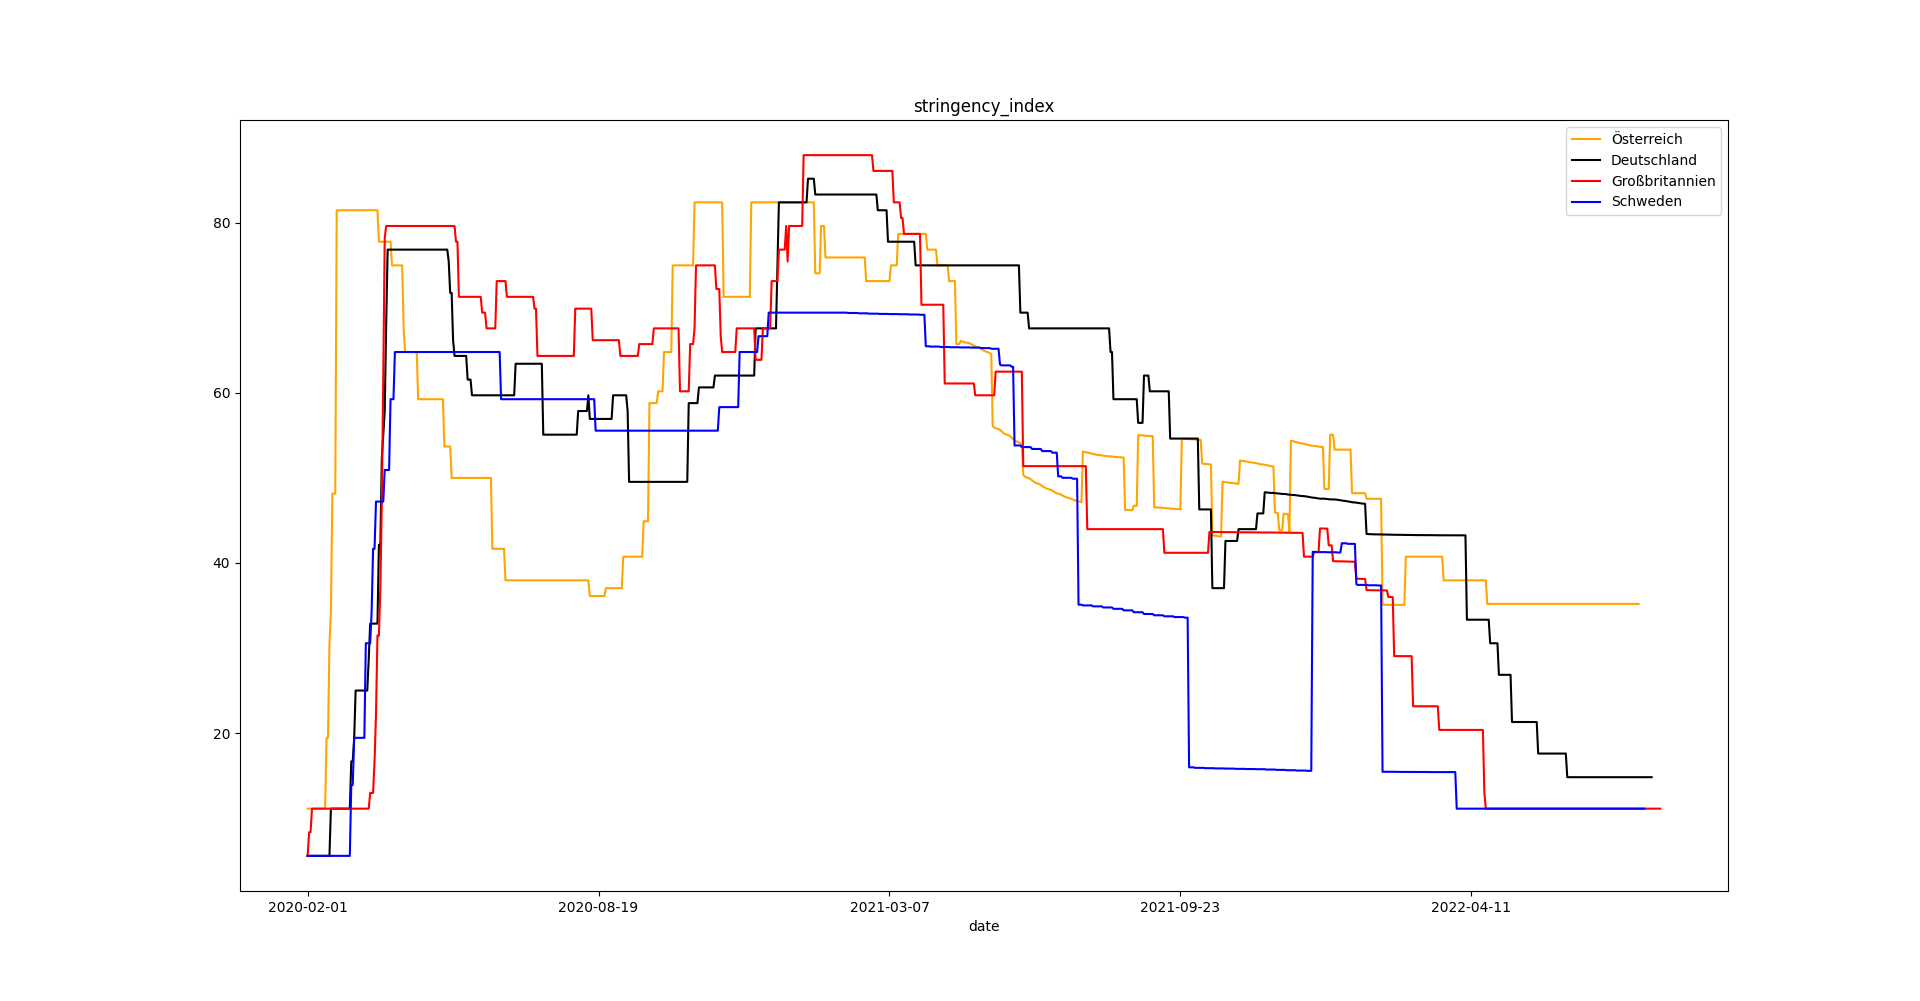
\includegraphics[trim={4cm 2cm 4cm 3cm},clip,width=\linewidth]{stringency_index_comparison2}
\end{figure}

Der Stringency Index korrelierte in jedem der untersuchten Staaten sowohl mit den Fallzahlen als auch mit den Todesfällen, wobei diese Korrelation nicht so stark wie erwartet und im Fall Großbritanniens sogar schwach ausgeprägt war.

Doch wie genau wurden Maßnahmen eingehalten? Dies lässt sich auch im Google Mobility Report beobachten - Besuche im Einzelhandel und Nutzung von Freizeitangeboten brach im ersten Lockdown um über 80\% ein, auch im öffentlichem Verkehr war ein Fahrgastzahlrückgang zu sehen - mit leichten Spitzen über die Weihnachtsfeiertage.
Interessant ist, dass allerdings in jedem Lockdown Familien- und Freundschaftsbesuche leicht zunahmen.
Im Arbeitsalltag lässt sich anhand der Daten beobachten, dass Home Office seit Pandemiebeginn zur Arbeitswelt dazugehört, hier sind Veränderungen zu sehen, die mit den aktuellen Fallzahlen einhergehen, eine Aktivität in den Büros wie vor der Pandemie wurde allerdings nicht mehr erreicht. \cite{google-mobility-report}

\begin{figure}[ht]
    \caption{Der Google Mobility Report zeigt die Umsetzung der Maßnahmen in Österreich}
    \label{fig:mobility_index_at}
    \centering
    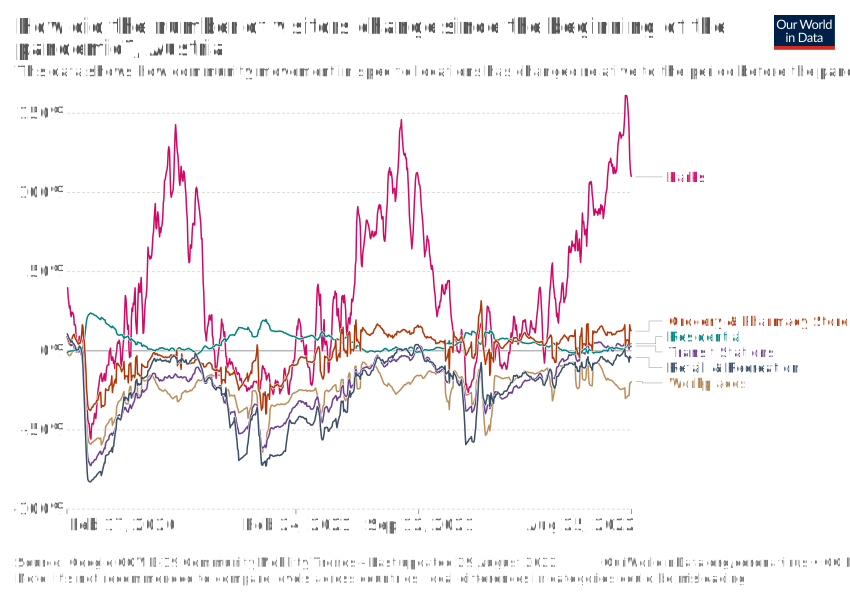
\includegraphics[trim={0 0 0 12cm},clip,width=\linewidth]{changes-visitors-covid-at}
\end{figure}

\subsection{Impfung gegen Sars-Cov-2}

Es konnte in jedem der untersuchten Länder eine starke Korrelation zwischen der Impfrate und den Fallzahlen bzw. den Todesfällen festgestellt werden. Diese war auch stärker als die Korrelation zwischen diesen Werten und dem Stringency Index.

\begin{figure}[ht]
    \caption{Neue Impfungen pro 100 Einwohner}
    \label{fig:vaccination_comparison}
    \centering
    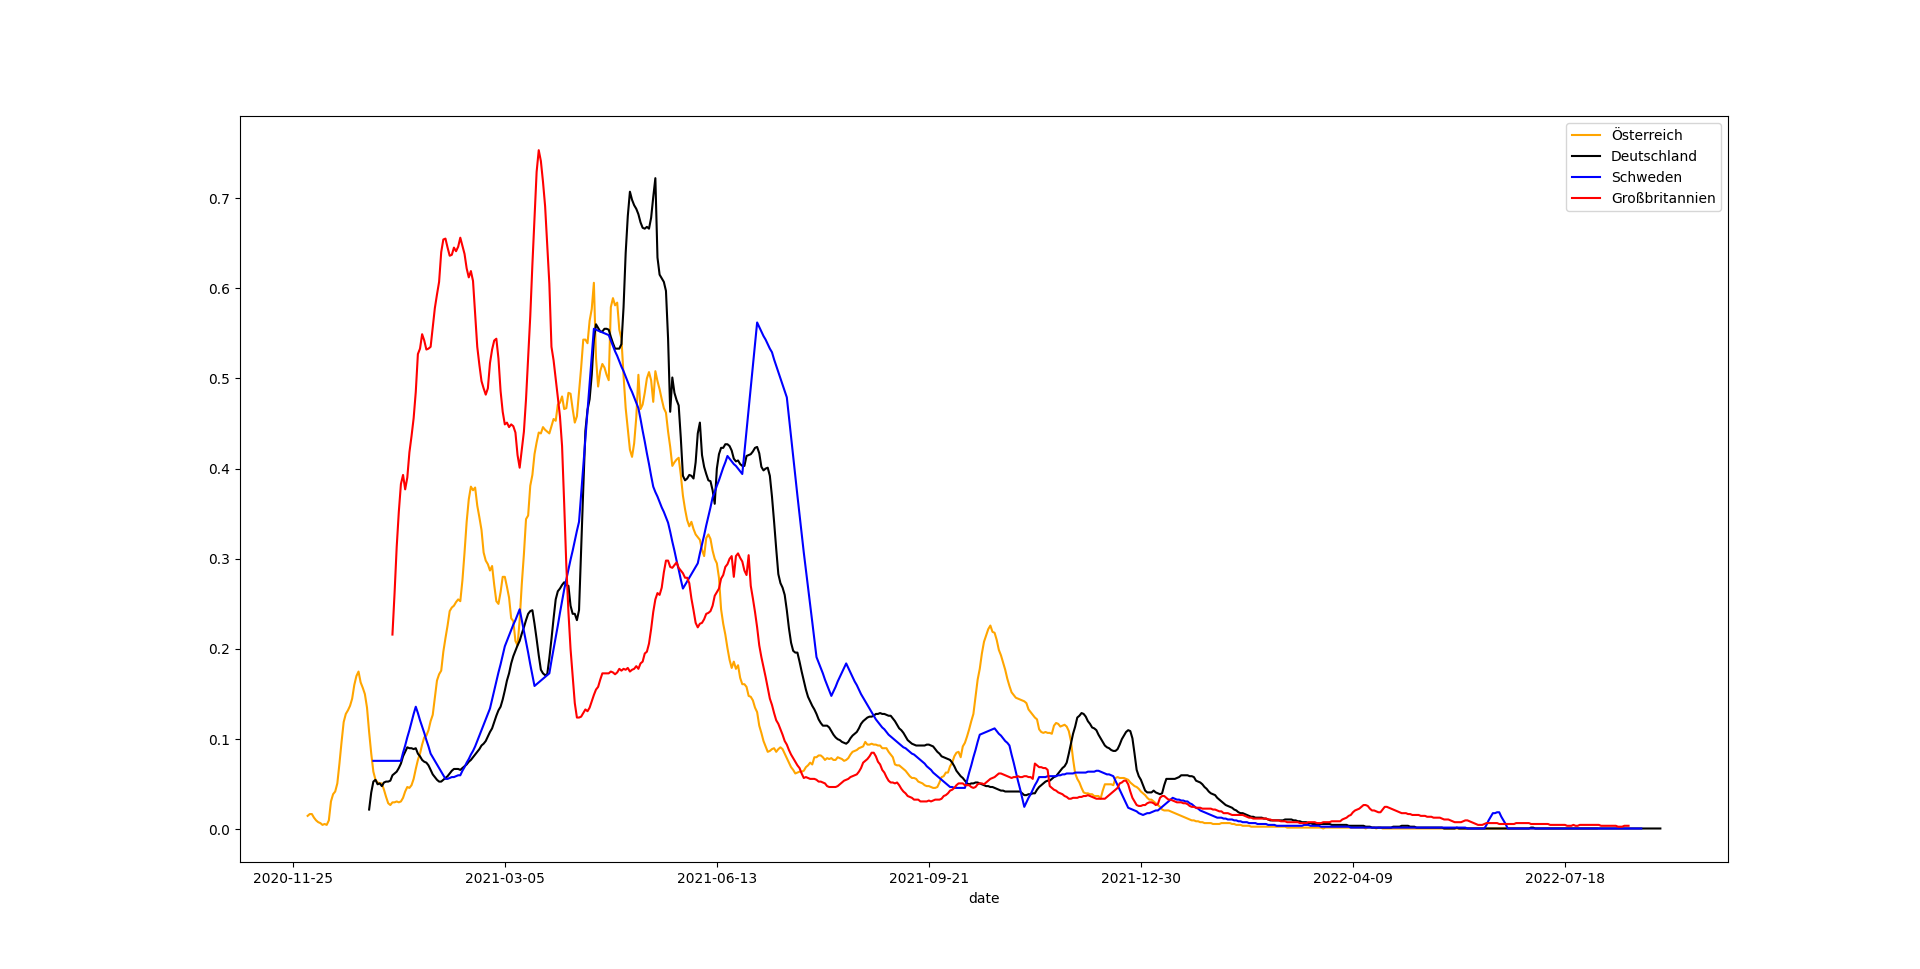
\includegraphics[trim={4cm 2cm 4cm 2,5cm},clip,width=\linewidth]{vacc_comparison2}
\end{figure}


\begin{figure}[ht]
    \caption{Fallzahlen pro Million Einwohner}
    \label{fig:cases_comparison}
    \centering
    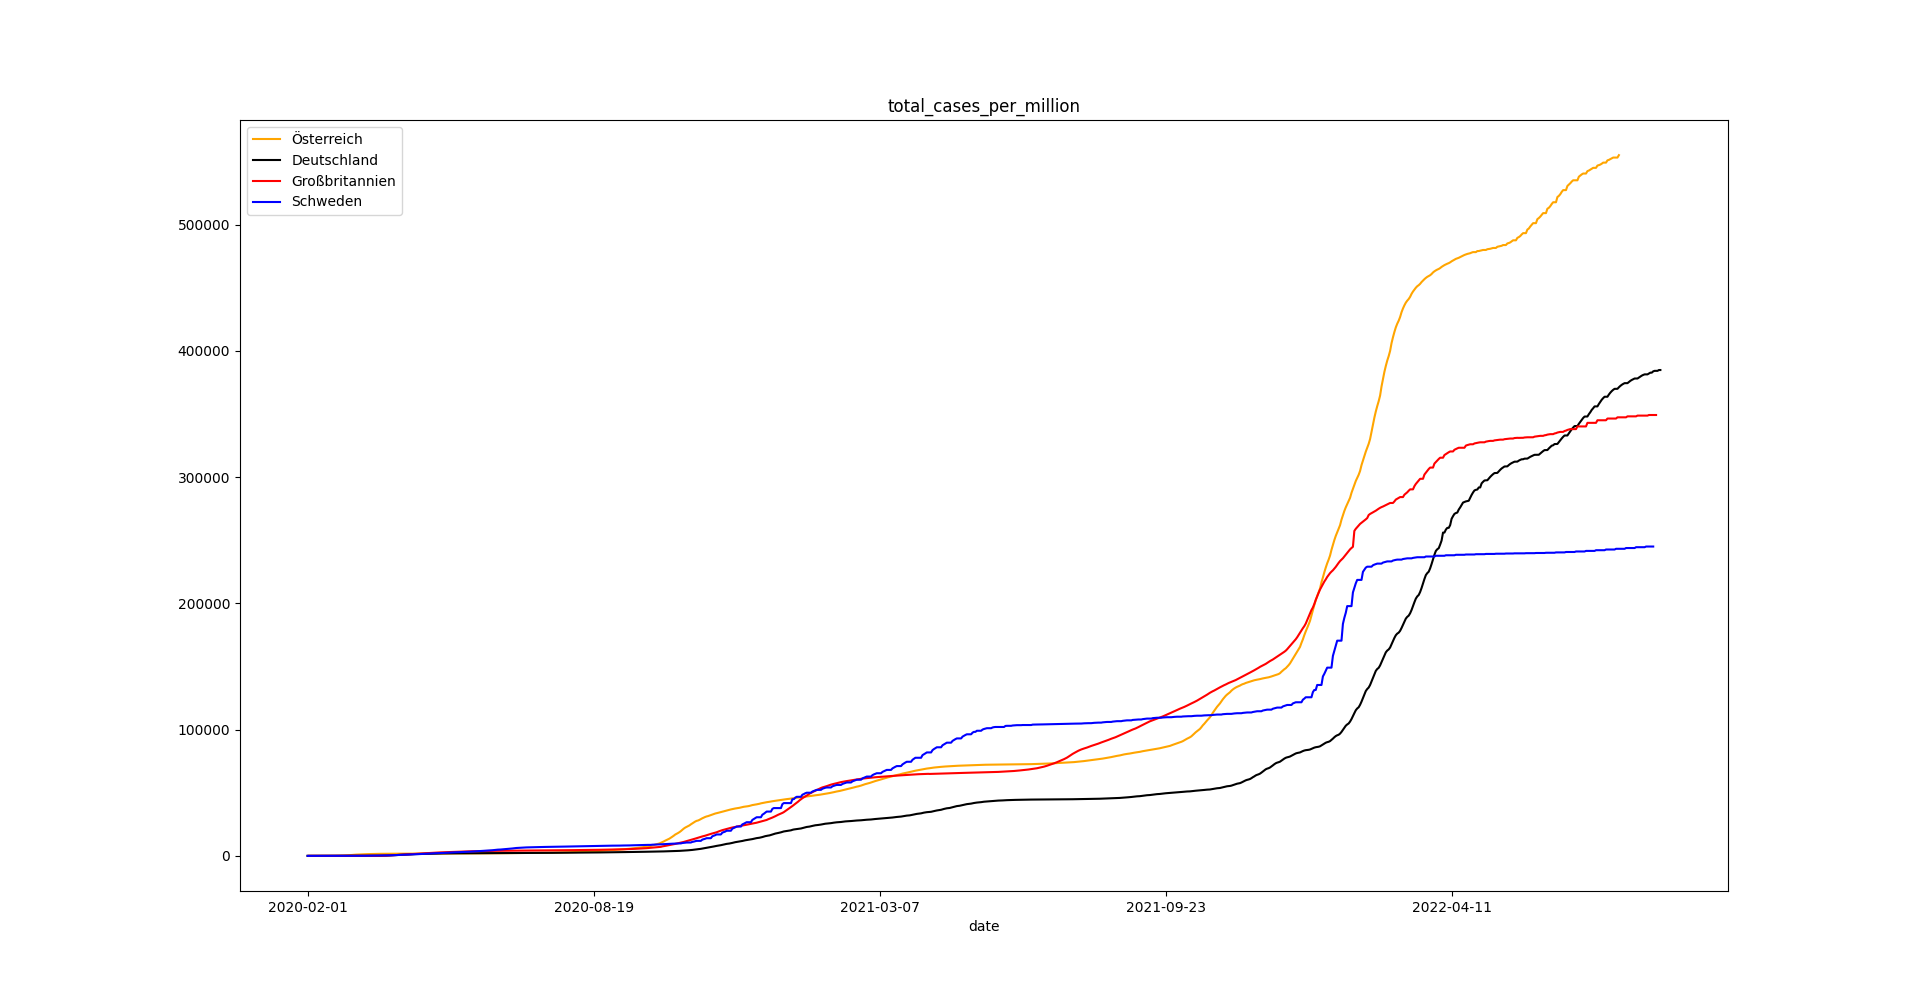
\includegraphics[trim={4cm 2cm 4cm 3cm},clip,width=\linewidth]{total_cases_comparison2}
\end{figure}


\begin{figure}[ht]
    \caption{Todesfälle pro Million Einwohner}
    \label{fig:death_comparison}
    \centering
    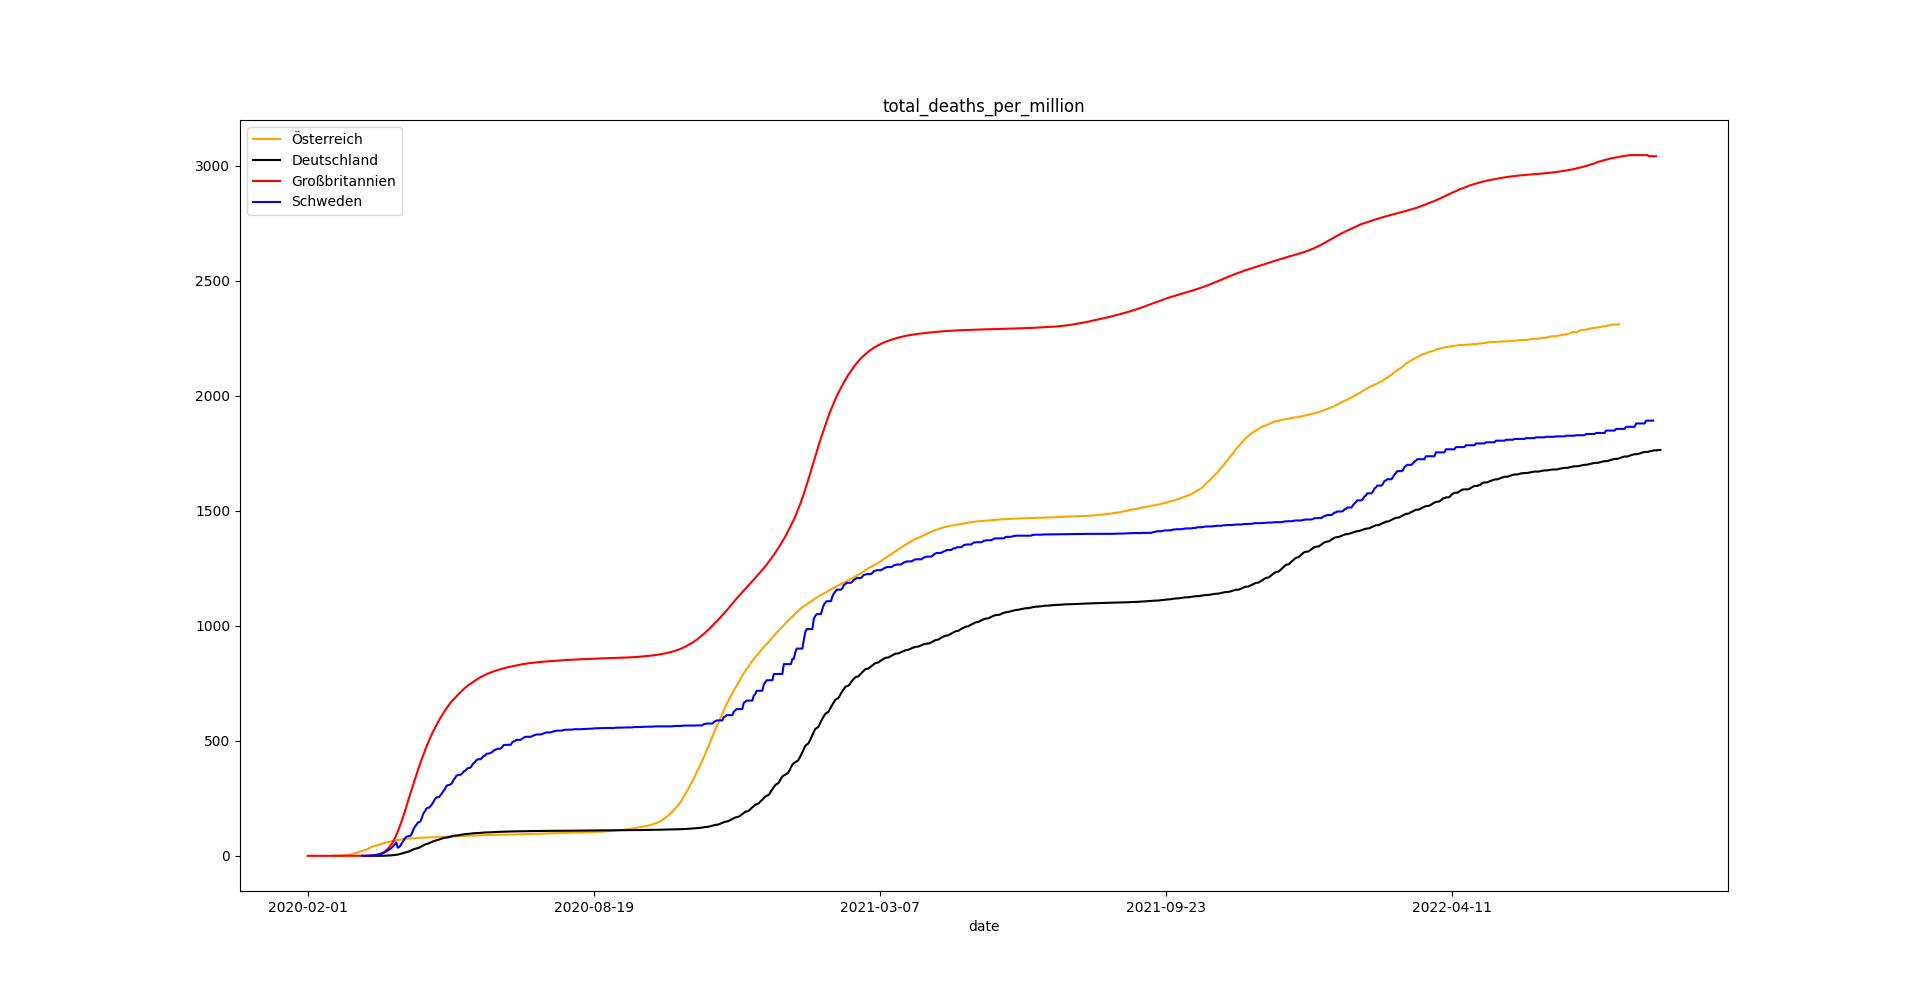
\includegraphics[trim={4cm 2cm 4cm 3cm},clip,width=\linewidth]{total_deaths_comparison2}
\end{figure}

\newpage

\section{Diskussion}

Es sind sowohl Korrelationen zwischen den Maßnahmen und den Fallzahlen als auch zwischen der Impfquote und den Fallzahlen zu beobachten. Interessant wäre eine Isolierung einzelner Maßnahmen. Dies gestaltete sich jedoch schwierig, da der Stringency Index bloß einen Anhaltspunkt bietet. Aus Deutschland liegen hierzu zwar sehr feingranulare Daten vorliegen, allerdings nie nur einzelne Maßnahmen, sondern immer ein Maßnahmenpaket erlassen wurde. In einer zukünftigen Arbeit könnten jedoch Daten aus einzelnen Bundesländern untersucht und verglichen werden. Eine alternative Herangehensweise könnte eine Untersuchung der Rohdaten des Stringency Index sein.

% /* cSpell:disable */